%%%%%%%%%%%%%%%%%%%%%%%%%%%%%%%%%%%%%%%%%%%%%%%%%%%%%%% 
% Preamble 
%%%%%%%%%%%%%%%%%%%%%%%%%%%%%%%%%%%%%%%%%%%%%%%%%%%%%%%

% Select build mode from:
%     quick - try to compile quickly (no extras)
%     debug - add grid lines/compile times
%     proof - local version of "final" 
%     final - Final publishable version (need LuaLaTeX)
%               NOTE: final should probably replace the documentclass to be 
% .                    PurdueThesis (not currently handled automatically) 
\def\ZZbuildmode{proof}

% Input arguments required by PurdueThesis

% ----------------- Author/Document Info -----------------
% Auuthor Name
\def\ZZauthor{Henri Poincar\'e}

% "May XXXX", "August XXXX", or "December XXXX"
\def\ZZgraduation{May 2023}

% Title
\def\ZZtitle{This is the Title}


% -------------------- Degree Program ---------------------
% Either:
%     Doctor of Philosophy
%     Master of Science in Aeronautics and Astronautics
\def\ZZdegree{Doctor of Philosophy}

% Either "A Dissertation" or "A Thesis"
\def\ZZdocument{A Dissertation}


% --------------- Final Draft Defaults (AAE) ---------------

% Purdue AAE (West Lafayette)
\def\ZZinstitution{Purdue University}
\def\ZZcampus{West\space Lafayette}
\def\ZZprogram{Aeronautics and Astronautics}

% Defaults for final draft
%      These are overwritten in PurdueThesisNL.cls but 
%      not in PurdueThesis.cls 
\def\ZZshowgridlines{false}
\def\ZZshowmarginlines{false}
\def\ZZshowtimestamp{false}
\def\ZZtodonotes{false}
\def\ZZatinformation{}
\def\ZZshowcolophon{false}
\def\ZZshowdiagonalline{false}

% Build the document (manually choose between official and local template)
% \documentclass{PurdueThesis}
\documentclass{PurdueThesisNL}

% Set up the latex document w/ imports, definitions, and template customizations
\ConfigureBibliography
% \graphicspath{{eps/}{tiff/}}
\graphicspath{{figures/}{figures/template}}

% Look in the "packages" subfolder for packages.
% This is done to reduce the number of files in the main thesis folder
% so the ones in there are easier to find.
\makeatletter
  \def\input@path{{packages/}}
\makeatother

% The vertical space between a table heading and the table contents in a tabular environment.
\newcommand{\tabularspace}{\noalign{\vspace*{2pt}}}

% Define boolean variables that contorl how the document is compiled
\newboolean{quick}
\newboolean{debug}
\newboolean{proof}
\newboolean{final}
\newboolean{quick-or-debug}
\newboolean{proof-or-final}

\ifthenelse{\equal{\ZZbuildmode}{quick}}
    {\setboolean{quick}{true}}{\setboolean{quick}{false}}
\ifthenelse{\equal{\ZZbuildmode}{debug}}
    {\setboolean{debug}{true}}{\setboolean{debug}{false}}
\ifthenelse{\equal{\ZZbuildmode}{proof}}
    {\setboolean{proof}{true}}{\setboolean{proof}{false}}
\ifthenelse{\equal{\ZZbuildmode}{final}}
    {\setboolean{final}{true}}{\setboolean{final}{false}}

\ifthenelse{\boolean{quick} \OR \boolean{debug}}
  {\setboolean{quick-or-debug}{true}}
  {\setboolean{quick-or-debug}{false}}
\ifthenelse{\boolean{proof} \OR \boolean{final}}
  {\setboolean{proof-or-final}{true}}
  {\setboolean{proof-or-final}{false}}

% -------------------- From Template -------------------

% So "_" will work in URLs when using BibTeX.
\usepackage[T1]{fontenc}

% The mathtools package
% (see http://mirror.utexas.edu/ctan/macros/latex/required/amsmath/amsmath.pdf)
% loads the amsmath package which defines the
%     align
%     align*
%     alignat
%     alignat*
%     equation
%     equation*
%     flalign
%     flalign*
%     gather
%     gather*
%     multitaper
%     multitaper*
%     split
% environments and extends amsmath by defining many other commands.
% See
%     https://ctan.org/pkg/amsmath
% for information about amsmath and
%     http://ctan.math.washington.edu/tex-archive/macros/latex/contrib/mathtools/mathtools.pdf
% for information about mathtools.
\usepackage{mathtools}

% Define \FigureDash.
% \FigureDash is a dash the width of a digit in the current font.
\usepackage{pa-figure-dash}

% For PurdueThesis, PuTh, TeX, LaTeX, METAFONT, METAPOST, etc. related logos.
\usepackage{pa-logos}

% (Or maybe use isomath instead?  -mark  2021-06-20)
% Follow ISO 80000-2:2019
%     o   put e, i, j, and pi in upright font automatically
%     o   use, for example, "\di x" to get "\,mathrm{d}\/x"
% This loads
%     o   amsmath.sty (which is already loaded above)
%     o   mathtools.sty
%     o   upgreek.sty
% Load the package.
\usepackage{pa-mismath}
    % Tell mismath to put e, i, j, and pi in upright font automatically.
    \enumber
    \inumber
    \jnumber
    \pinumber
  % To typeset math italic e, i, j, and pi use
  %     \mathit e
  %     \mathit i
  %     \mathit j
  %     \itpi


% Define \FloatBarrier
\usepackage{placeins}

% For highlighting text using \hl
\usepackage{soul}

% For \sfrac, used to do slanted fractions, similar to, e.g., 1/2, but 1 is small and high and 2 is small and low.
\usepackage{xfrac}

% For typographical conventions stuff including
%     \Emph{...}
%     \First{...}
%     \Keys{...}
%     \Literal{...}
%     \Menu{...}
%     \Place{...}
%     \Shell{...}
% This must be after
%     \usepackage{tikz}
\usepackage{pa-typographic-conventions}


% ----------------- Added Dependencies -----------------

% Generate lorem ipsum 
%    e.g.: \lipsum[1-2]
\usepackage{lipsum}



% cleveref
%   For easier cross-referencing
%   Redefine the subref formatting so that you get:
%     Figure 1.1(a) instead of Figure 1.1a
\usepackage[noabbrev, capitalise]{cleveref}
  \captionsetup[subfigure]{subrefformat=simple,labelformat=simple}
  \renewcommand\thesubfigure{(\alph{subfigure})}

% Put table captions on top / adjust the spacing
\captionsetup[table]{
    position=above,
    belowskip=4pt
  }
% \usepackage[skip=3.5\baselineskip]{caption}
% \captionsetup[table]{0.5\baselineskip}
% \captionsetup[table]{skip=90pt}
% \usepackage{float}
%   \floatstyle{plaintop}
%   \restylefloat{table}


% Define \NL (newline) so LaTeX goes to the next output line.
% Just doing \\ complains
%     ! LaTeX Error: There's no line here to end.
% \mbox{} is an empty math box.
\newcommand{\NL}{\mbox{}\\}

% TODO: not sure if everything should use \input

%%%%%%%%%%%%%%%%%%%%%%%%%%%%%%%%%%%%%%%%%%%%%%%%%%%%%%% 
% Ducument 
%%%%%%%%%%%%%%%%%%%%%%%%%%%%%%%%%%%%%%%%%%%%%%%%%%%%%%% 

\begin{document}
\maketitle

% Front matter (title, acknowledgements, abstract, etc)

% Only include these sections if this is a proof or final version
\ifthenelse{\boolean{proof-or-final}}{
    % Statement of Thesis/Dissertation Approval Page
% This page is REQUIRED.  The page should be numbered "2"
% and should NOT be listed in your TABLE OF CONTENTS.

\begin{statement}
    % Delete or add \entry commands as needed for all committe members.
    \entry{Dr.~Kathleen C. Howell, Chair}{School of Aeronautics and Astronautics}
    \entry{Dr.~Carolin Frueh}{School of Aeronautics and Astronautics}
    \entry{Dr.~Dengfeng Sun}{School of Aeronautics and Astronautics}
    \entry{Dr.~James M. Longuski}{School of Aeronautics and Astronautics}
    % There should be one \approvedby command containing the
    % "FORM 9 THESIS FORM HEAD NAME HERE" (from TEMPL, retrieved on 2020-03-01).
    \approvedby{Dr.~Gregory A. Blaisdell}
\end{statement}

  
    % Dedication page is optional.
% A name and often a message in tribute to a person or cause.
% References: WEB9 332.

\ifthenelse{\boolean{quick-or-debug}}{}
{
\begin{dedication}
    Here is my dedication
\end{dedication}
}
    % Acknowledgements page is optional but most theses include
% a brief statement of appreciation or recognition of special
% assistance.
\ifthenelse{\boolean{quick-or-debug}}{}
{
\begin{acknowledgments}
    Purdue University's Engineering Computer Network
    and Graduate School helped fund \PurdueThesisLogo\ development.
\end{acknowledgments}
}
    % The preface is optional.
% References: TCMOS17 1.49, WEB9 927.

% \begin{preface}
%   This is the preface.
% \end{preface}
    %
    \pdfbookmark{TABLE OF CONTENTS}{Contents}
    \tableofcontents
    \listoftables
    \listoffigures
}{}

% Optional: Symbols, Abbreviations, Nomenclature, Glossary

% Always include the abstract
\begin{abstract}%
    \PurdueThesisLogo\ is a \LaTeX\ document class used for
    master's bypass reports,
    master's theses,
    PhD dissertations,
    and PhD preliminary reports.
    This template demonstrates how to use \PurdueThesisLogo.
  
  \end{abstract}
  

% Input all chapters here

\chapter{INTRODUCTION}
Experimenting with the available typographic conventions defined in the Purdue file: \NL \Literal|pa-typographic-conventions.sty|:  these include \Emph{Emph} \First{First} \First{Title} \Keys{Keys} \Literal|Literal| \Menu{Menu} \Menu{Open menu > Preferences} \Shell{Shell.sh}. Now let's try out a footnote\footnote{I'm a footnote!}, one of the fancy TODO notes  \todocomment{Do I really need this?}, and more scary TODO \todowarn{Be careful here}, as well as a a todo error \todoerror{This is wrong!} as well as a citation \cite{Howell:1984_HaloOrbits}. Note the TODO comments currently only show up in \Literal|quick| or \Literal|debug| modes (for now).


\section{Subcaption / Cleveref Testing}
Here is a very important and informative figure for Orion. You can see in \cref{fig:orion} that there is both \cref{fig:orion:a} and \cref{fig:orion:b}! There is also important information in \cref{tab:sample_table}. If you're confused, then \cref{eq:euler} should clarify things. Some other ways to put it: \cref{eq:euler,eq:pythagorean} and \cref{eq:euler,eq:pythagorean,eq:calculus}. 

\begin{figure}[p]
    \centering
    \begin{subcaptionblock}{.49\textwidth}
        \centering
        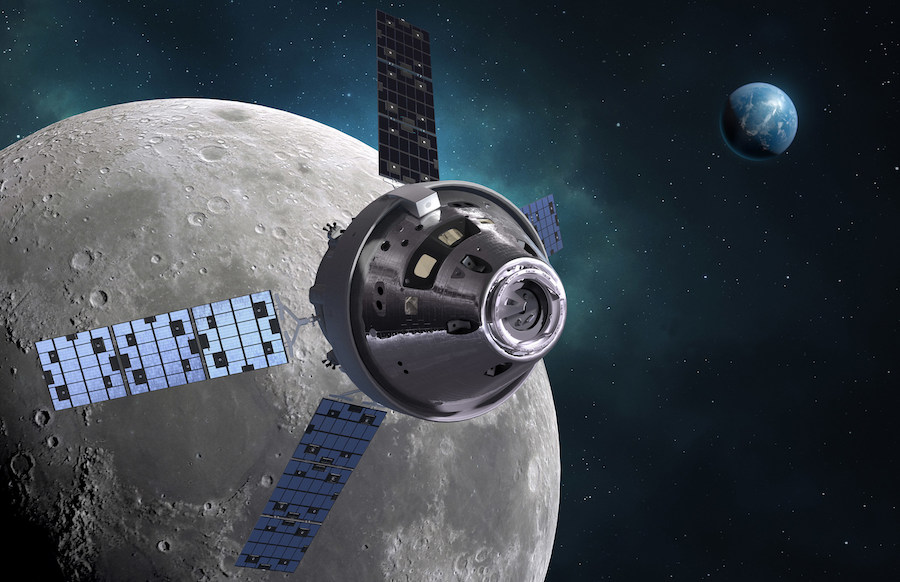
\includegraphics[width=\textwidth]{orion1}
        \caption{Orion 1}
        \label{fig:orion:a}
    \end{subcaptionblock} %
    \begin{subcaptionblock}{.49\textwidth}
        \centering
        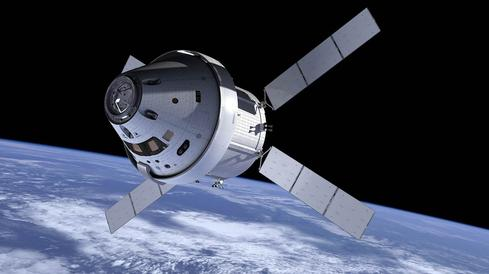
\includegraphics[width=\textwidth]{orion2}
        \caption{Orion 2}
        \label{fig:orion:b}
    \end{subcaptionblock} %
    \caption{Two images of Orion: \subref{fig:orion:a} and \subref{fig:orion:b}.}
    \label{fig:orion}
\end{figure}

\begin{table}[p]
    \centering
    \caption{Sample Table}
    \begin{tabular}{|c|c|}
    \hline
        Sample & Table\\
        $x$ & 2\\
    \hline
    \end{tabular}
    \label{tab:sample_table}
\end{table}

\subsection{Important Math}

\begin{equation}
    e^{i\pi}+1=0
    \label{eq:euler}
\end{equation}

\begin{equation}
    a^2+b^2=c^2
    \label{eq:pythagorean}
\end{equation}

\begin{equation}
    \frac{df}{dt} = \lim_{h\rightarrow 0} \frac{f(t+h)-f(t)}{h}
    \label{eq:calculus}
\end{equation}

\subsection{Numbers/Units}
Some of the number formats available: \num{-e10}. \numproduct{2 x 4}. \numrange{10}{11}. \ang{12.3}.

Experimenting with the siunits package: 8 \unit{\kilo\gram\metre\per\square\second}. 9\unit{\newton}. \qty{2.3e27}{\kilogram}. \qty[per-mode = fraction]{1,345}{\coulomb\per\mole}.

\subsubsection{A subsubsection} 
A subsubsection for testing out the table of contents

\paragraph{A paragraph}
What happens for a paragraph in the table of contents?
\chapter{BACKGROUND}
Background information etc
% ...

% Appendices

% Use ``\appendix'' for one appendix or ``\appendices'' for more than one appendix.
\appendices

% A vita is optional for masters theses
% and required for doctoral dissertations.
% Reference: TM2017 page 13.

\begin{vita}
  [Put a brief autobiographical sketch here.]
\end{vita}
    

% Back content (vita, bib settings, etc.)

% -------------------- From Template -------------------
  
%
% This is only done if you are using BibLaTeX.
%
% \makeatletter  % commented out on 2022-01-26
%   \defbibenvironment{bibliography}
%     {%
%       \list
%         {%
%           \printtext[labelnumberwidth]%
%           {%
%             \printfield{prefixnumber}%
%             \printfield{labelnumber}%
%           }%
%         }%
%         {%
%           \setlength{\bibhang}{1in} %%%%% was 0pt
%           \setlength{\itemindent}{1in}%  -\leftmargin} %%%%% was 0pt
%           \setlength{\itemsep}{\bibitemsep}%
%           \setlength{\leftmargin}{0pt}%  .22in} % 0.42in}
%           \setlength{\parsep}{\bibparsep}%
%            \setlength{\rightmargin}{0.33in}%
%         }%
%     }
%     {\endlist}
%     {\item}
% \makeatother  % commented out on 2022-01-26



% \immediate\setlength{\labelnumberwidth}{1.5in} %%%%% was commented out
\setlength{\labelwidth}{1.5in}
\def\sllnsez{[999] }

{%
  % Make _ in URLs visible.
  % \def\t{\char'137}%
  \catcode`*=\active
  \def*{\char'137}%  \char'137 is _
  \PrintBibliography
}

\end{document}
